\textual

% ----------------------------------------------------------
% Introdução
% ----------------------------------------------------------
% ----------------------------------------------------------
% Introdução (exemplo de capítulo sem numeração, mas presente no Sumário)
% ----------------------------------------------------------
\chapter{Introdução}
\label{chap:intro}
% ----------------------------------------------------------

A inteligência artificial (IA) vem ganhando manchetes no mundo todo, sendo anunciada tanto como uma salvação econômica quanto como precursora de desintegração social. Quando computadores programáveis foram concebidos pela primeira vez, as pessoas se perguntavam se essas máquinas poderiam se tornar inteligentes, mais de cem anos antes de uma ser construída %.
\cite{menabrea1843sketch}.
 Hoje, a inteligência artificial é um campo com inúmeras aplicações práticas e tópicos de pesquisa ativos. Buscamos softwares inteligentes para automatizar o trabalho de rotina, entender a fala ou as imagens, fazer diagnósticos em medicina e apoiar a pesquisa científica \cite{Goodfellow-et-al-2016}.


A IA adiciona inteligência a produtos existentes. Na maioria dos casos, a inteligência artificial não é vendida como uma aplicação individual. Pelo contrário, produtos já existentes são aprimorados com funcionalidades de IA, de maneira parecida como a Siri foi adicionada aos produtos da \textit{Apple}. Automação, plataformas de conversa, robôs e aparelhos inteligentes podem ser combinados com grandes quantidades de dados para aprimorar diversas tecnologias para casa e escritório, de inteligência em segurança à análise de investimentos.

A maioria dos exemplos de IA sobre os quais se ouve falar hoje – de computadores mestres em xadrez a carros autônomos – dependem de \textit{deep learning} e processamento de linguagem natural (PNL) \cite{pln-o-que-e}. Treinar um agente para superar os jogadores humanos e otimizar sua performance pode nos ensinar como otimizar diferentes processos em uma grande variedade de situações. Foi o que o \textit{DeepMind} do Google fez com seu popular \textit{AlphaGo} e seu sucessor \textit{AlphaZero}, vencendo os campeões mundiais em Go, xadrez e shogi, e obtendo resultados de performance nunca antes vistos.

\section{Motivação}

Técnicas de aprendizado de máquina e algoritmos de \textit{deep learning} têm consistentemente melhorado a capacidade de um computador de fornecer reconhecimento de padrões e previsões cada vez mais precisas. Além disso, sistemas de DL são consistentemente aplicados com sucesso a conjuntos de aplicações cada vez mais amplos.

Ao mesmo tempo em que a escala e a precisão das redes neurais aumentaram, a complexidade das tarefas que podem ser resolvidas também cresceu significativamente. 
Uma conquista importante de sistemas de DL é a sua extensão ao domínio da aprendizagem por reforço ou \textit{reinforcement learning} (RL) \cite{reinforcement-learning-intro-2018}. No contexto do aprendizado por reforço, um agente autônomo deve aprender a executar uma tarefa por tentativa e erro, sem nenhuma orientação do operador humano. 

Além do valor para pesquisa em múltiplas áreas da ciência, muitas dessas aplicações de aprendizado de máquina e \textit{deep learning} são altamente lucrativas. O aprendizado de máquina hoje é usado por muitas empresas de tecnologia, incluindo \textit{Google, Microsoft, Facebook}, IBM, \textit{Baidu, Apple, Adobe, Netflix}.

Diante à crescente presença de sistemas que utilizam técnicas de \textit{deep learning} no dia-a-dia, nota-se o grande potencial do investimento em pesquisa, modelagem de novos problemas e estudo de técnicas de aprendizado de máquina. 
%
Uma interessante aplicação desses sistemas está na área de jogos digitais. A indústria de videogames tem testemunhado um enorme crescimento, graças, em boa parte, ao incrível aumento no poder da computação em termos de representações visuais. 
%
%
Seja no controle de personagens não-jogadores (NPC), ou para a geração de conteúdo processual (PCG), são inúmeras as potenciais aplicações dessas técnicas em jogos digitais.
%
O potencial dessas ferramentas de obter uma vantagem competitiva no mercado, ou simplesmente fornecer uma melhor experiência para o usuário é, no mínimo, instigante.
%
Nesse contexto, a modelagem de novos problemas, implementação de soluções utilizando técnicas de \textit{deep learning} e investimento na área, torna-se uma relevante contribuição para o estado da arte.


\section{Objetivos}
 O presente trabalho tem como objetivo geral propor o desenvolvimento de uma IA capaz de aprender a jogar diferentes jogos, desde que se tenha acesso ao código fonte e feito em Allegro. Para isso, será implementado um algoritmo utilizando \textit{Deep Reinforcement Learning} (DRL), abordagem que consiste em fornecer ao sistema parâmetros relacionados ao seu estado e uma recompensa positiva ou negativa com base em suas ações. 
 Nenhuma regra sobre o jogo é dada e, inicialmente, a IA não tem informações sobre o que precisa fazer. A única informação passada para a IA são os comandos básicos do jogo. 
 O objetivo do sistema é descobrir e elaborar uma estratégia para maximizar a pontuação - ou a recompensa.
 % Diferente de muitas IAs que focam na solução de um único problema, a proposta deste projeto é elaborar uma IA que seja genérica e capaz solucionar e elaborar estratégias para uma variedade de situações diferentes.

 Os objetivos mais específicos deste trabalho são:
 \begin{enumerate}
 	\item Revisão da literatura do problema;
 	\item Descrição e modelagem do problema;
 	\item Proposta de critérios adicionais que possibilitem estimar outras características das possíveis soluções do projeto, tais como performance, confiabilidade, entre outras;
 	\item Proposta de um algoritmo de \textit{deep learning} para a solução do problema;
 	\item Análise dos resultados obtidos em comparação com diferentes soluções implementadas por outras entidades e utilizadas na prática por empresas atuando no mercado.
 \end{enumerate}

 Perante o exposto, a implementação de algoritmos que utilizam o aprendizado de máquina de forma a serem aplicados em diferentes cenários,
 apresenta um potencial de propor novas estratégias e otimizar sistemas já existentes, melhorar a qualidade do produto final e a experiência do usuário, além de proporcionar uma vantagem competitiva no mercado.

\section{Descrição do problema}
\label{sec:descricao_do_problema}
O campo da inteligência artificial é capaz de solucionar, com certa facilidade, problemas que são intelectualmente muito difíceis para os serem humanos, mas relativamente diretos para os computadores - problemas que podem ser descritos por uma lista de regras formais e matemáticas. Tarefas abstratas e formais que estão entre os empreendimentos mentais mais difíceis para um ser humano estão entre os mais fáceis para um computador.

Ironicamente, o grande desafio à inteligência artificial provou estar em resolver tarefas fáceis de executar para um ser humano. Problemas  que parecem automáticos, que resolvemos intuitivamente, como reconhecer palavras faladas ou rostos em imagens. Os computadores há muito conseguem derrotar até o melhor jogador de xadrez humano \cite{Hsu:2002:BDB:601291}, mas apenas recentemente começaram a alcançar algumas das habilidades dos seres humanos comuns, como reconhecer objetos ou fala. 

A vida cotidiana de uma pessoa requer uma imensa quantidade de conhecimento sobre o mundo. A grande quantidade de informação desses cenários torna inviável a codificação de todas as regras do sistema e, por isso, o computador tem uma grande dificuldade para solucionar esses problemas. Além disso, grande parte desse conhecimento é subjetivo e intuitivo e, portanto, difícil de articular de maneira formal. Os computadores precisam capturar esse mesmo conhecimento para se comportarem de maneira inteligente. Um dos principais desafios da inteligência artificial é como obter esse conhecimento informal em um computador.

As dificuldades enfrentadas por sistemas que dependem de conhecimento codificado sugerem que os sistemas de IA necessitam da capacidade de adquirir seu próprio conhecimento, extraindo padrões de dados brutos. Esse recurso é conhecido como aprendizado de máquina ou \textit{machine learning} (ML). A introdução do aprendizado de máquina permitiu que os computadores resolvessem problemas que envolvem o conhecimento sobre o mundo real e tomassem decisões mais subjetivas.


 O problema proposto nesse trabalho é o de implementar uma IA que, utilizando algoritmos de \textit{deep reinforcement learning}, seja capaz de aprender e desenvolver estratégias para jogar diferentes jogos digitais. Os requisitos do sistema podem ser resumidos pelos seguintes critérios:
\begin{enumerate}
	\item O sistema receberá, inicialmente, somente os comandos básicos do jogo. Nenhuma regra sobre o jogo é dada e, inicialmente, o agente não tem nenhuma informação sobre o que precisa fazer;

	\item O agente deve ser capaz de elaborar uma estratégia para maximizar sua pontuação e que alcance resultados consideravelmente superiores aos de uma abordagem aleatória e próximos aos de um agente humano;

	\item O sistema deverá ser capaz de lidar com cenários aleatórios, onde os obstáculos mudam a cada partida, e não aleatórios, onde os obstáculos são ``fixos'' e a dificuldade varia de acordo com o progresso no jogo;

	\item O sistema deve ser generalizado para que possa ser aplicado à diferentes cenários e treinado para jogar diferentes jogos digitais.
\end{enumerate}

De modo a garantir a factibilidade da implementação do sistema, algumas restrições devem ser acatadas. Por exemplo, além de haver a necessidade de se conhecer os comandos básicos do jogo, o sistema precisa ser capaz de obter informações atualizadas sobre o estado do jogo em que se encontra. No caso deste trabalho, foram definidas as seguintes restrições:

\begin{enumerate}
	\item O sistema deve ter acesso ao código fonte do jogo no qual será aplicado;
	\item O jogo deverá ter sido implementado em \textit{Allegro}\footnote{O acesso ao código fonte nos permite ter conhecimento dos comandos básicos do jogo, enquanto a biblioteca \textit{Allegro} fornece rotinas de baixo nível comumente necessárias na programação de jogos \cite{allegro}. Essas rotinas, por serem fáceis de manipular, auxiliarão na implementação de um sistema de aprendizado.};
	\item O jogo deve ser 2D para garantir a viabilidade da implementação do sistema.
\end{enumerate}

O desafio nesse projeto é criar e treinar uma rede neural convolucional capaz de aprender políticas através de pixels brutos em ambientes complexos por meio de um algoritmo de \textit{deep reinforcement learning}. O objetivo principal é implementar um agente que seja capaz de aprender a jogar o maior número de jogos possíveis sem conhecimento prévio do ambiente. Em outras palavras, o sistema deverá ser genérico e o agente não receberá nenhuma informação prévia sobre um jogo específico.
% subsection aplicação_de_drl_no_treinamento_de_uma_ia_para_aprender_a_jogar_jogos_em_allegro (end)

\section{Revisão da literatura}

Apesar de se falar sobre \textit{deep learning} como uma emocionante nova tecnologia, este tem uma história longa e rica, mas apresentando diversos nomes, os quais refletem diferentes pontos de vista filosóficos. Em termos gerais, ocorreram três ondas de desenvolvimento com níveis de popularidade variados: DL conhecido como \textit{cybernetics} nas décadas de 1940 a 1960, DL conhecido como \textit{connectionism} entre as décadas de 1980 e 1990 e o ressurgimento atual sob o nome de aprendizado profundo ou \textit{deep learning} a partir de 2006 \cite{Goodfellow-et-al-2016}.

Alguns dos primeiros algoritmos de aprendizado que são reconhecidos hoje pretendiam ser modelos computacionais de aprendizado biológico, isto é, modelos de como o aprendizado acontece ou pode acontecer no cérebro. Como resultado, um dos nomes que o DL passou é o de \textit{artificial neural networks} (ANNs). No entanto, o termo moderno ``\textit{deep learning}'' vai além da perspectiva neurocientífica da atual geração de modelos de aprendizado de máquina. Ele apela a um princípio mais geral de aprendizado de vários níveis de composição, que podem ser aplicados em estruturas de aprendizado de máquina que não são necessariamente inspiradas em neurônios.


Uma das muitas contribuições do DL está no reconhecimento de fala \cite{nassif:speech-rec:2019}. Até recentemente, os de reconhecimento automático de fala (ASR) combinavam principalmente modelos ocultos de Markov (HMMs) e modelos de mistura gaussianos (GMM). Com a introdução de redes neurais e, posteriormente, modelos de DL cada vez maiores e mais profundos e conjuntos de dados muito maiores, a precisão do reconhecimento foi dramaticamente aprimorada usando redes neurais para, eventualmente, substituir GMMs na tarefa de associar recursos acústicos a fonemas \cite{Goodfellow-et-al-2016}.


O \textit{deep learning} também contribuiu para outras ciências. As redes convolucionais modernas para reconhecimento de objetos e visão computacional fornecem um modelo de processamento visual com diversas aplicações na medicina \cite{Yeung:comp-vis:2019,dicarlo-afrax-yamins:2014}. O \textit{deep learning} também fornece ferramentas úteis para processar grandes quantidades de dados e fazer previsões úteis em campos científicos. Ele tem sido usado com sucesso para prever como as moléculas irão interagir, a fim de ajudar as empresas farmacêuticas a projetar novos medicamentos \cite{dahl2014multitask}, a procurar partículas subatômicas \cite{baldi:s:w:2015}, e para o processamento de linguagem natural \cite{Young_2018}. Espera-se que o DL apareça em cada vez mais campos científicos no futuro.

Pesquisas recentes em IA deram origem a técnicas poderosas para o \textit{deep reinforcement learning}. 
Na combinação de aprendizado de representação com comportamento orientado por recompensas, o DRL parece ter um interesse inerente à psicologia e neurociência. 
Um argumento contra essa abordagem foi o de que os procedimentos de aprendizado por DRL exigem grandes quantidades de dados de treinamento, sugerindo que esses algoritmos podem diferir fundamentalmente daqueles subjacentes ao aprendizado humano. 
Embora essa preocupação se aplique à onda inicial de técnicas de RL profunda, o trabalho subsequente de IA estabeleceu métodos que permitem que os sistemas de RL profunda aprendam mais rápida e eficientemente \cite{Botvinick:rl-fastandslow:2019}.

A IA em jogos digitais possui algumas peculiaridades \cite{Yannakakis:2012:GAR:2212908.2212954, Millington:2009:AIG:1795711}, que a distinguem da IA clássica, especialmente porque, em muitos casos, ela deve lidar com aplicativos em tempo real e não necessariamente precisa otimizar resultados. Ela pode ser explorada para muitos propósitos, que podem ser coletados em três macro-categorias principais: ajudar na jogabilidade, melhorar a imersão do jogador no mundo do jogo (também simular a psicologia dos agentes que representam os personagens que não jogam - NPCs) e apoiar o trabalho de designers de jogos e níveis \cite{Piergigli:drl:2019}. 
Entre as técnicas de IA mais difusas, podemos contar aquelas usadas para gerar procedimentalmente conteúdos \cite{Karavolos:automated-level-design:2018,Ripamonti2017} e aquelas destinadas a apoiar o sistema de tomada de decisão dos agentes artificiais \cite{Ripamonti:Believable-group-behaviours:2017}.

O aprendizado de máquina e as redes neurais são aplicadas aos jogos há muito tempo, mas seu uso recentemente conheceu um interesse renovado e aborda uma ampla variedade de tópicos.
No entanto, o uso dessas técnicas para treinar agentes em ambientes complexos, com várias ações simultâneas possíveis é um resultado bastante desafiador a ser alcançado \cite{Piergigli:drl:2019}.

Recentemente, o \textit{DeepMind} do Google desenvolveu o \textit{Deep Q-network} (DQN), uma arquitetura de rede neural, que demonstrou ser capaz de aprender políticas de controle no nível humano em vários jogos diferentes do Atari 2600 \cite{mnih-human-control-drl}. Os DQNs aprendem a estimar os valores Q (função de valor da ação do estado) de selecionar cada ação do estado atual do jogo. Como a função de valor da ação do estado é uma representação suficiente da política do agente, um jogo pode ser jogado selecionando a ação com o valor Q máximo em cada etapa do tempo. Dessa forma, aprendendo políticas de pixels em tela bruta a ações, essas redes têm demonstrado desempenho avançado em vários jogos do Atari 2600. Vale ressaltar que a mesma rede pode ser usada em várias tarefas sem nenhuma alteração e que o aprendizado é de ponta a ponta, dos valores brutos dos pixels aos valores Q, sem a necessidade de intervenção humana. Recentemente, DQNs foram estendidos para obter melhor desempenho em jogos ainda mais complexos \cite{Debidatta:playing-games-drl:2016}.




\section{Organização do trabalho} % (fold)
\label{sec:organização_do_trabalho}
Este trabalho está estruturado em cinco capítulos. O \textbf{Capítulo \ref{chap:intro}} consiste em uma breve introdução ao tema do projeto e uma análise da literatura do problema. O \textbf{Capítulo \ref{chap:ctx-hum}} apresenta uma contextualização do problema nos âmbitos social, ambiental e econômico. O \textbf{Capítulo \ref{chap:abordagem}} discorre a abordagem proposta para o problema, assim como sua respectiva modelagem matemática. O \textbf{Capítulo \ref{chap:conclusoes}} encerra o trabalho com as conclusões e apresenta as propostas de continuidade para o Trabalho de Conclusão de Curso II.

% section organização_do_trabalho (end)




% ---

% ----------------------------------------------------------
% Contextualização em Humanidades
% ----------------------------------------------------------
% ----------------------------------------------------------
% Contextualização em Humanidades
% ----------------------------------------------------------
\chapter{Contextualização em Humanidades}
\label{chap:ctx-hum}
% ----------------------------------------------------------


Nos últimos anos, houve um progresso significativo na solução de problemas desafiadores em diversos campos, utilizando algoritmos de \textit{deep reinforcement learning}. Como consequência, o RL experimentou um crescimento dramático na atenção e no interesse da comunidade científica. A \textbf{Figura \ref{rl-publications-overview}} mostra o crescimento no número de publicações relacionadas à RL nos últimos 30 anos.

\begin{figure}[h]
  \centering
  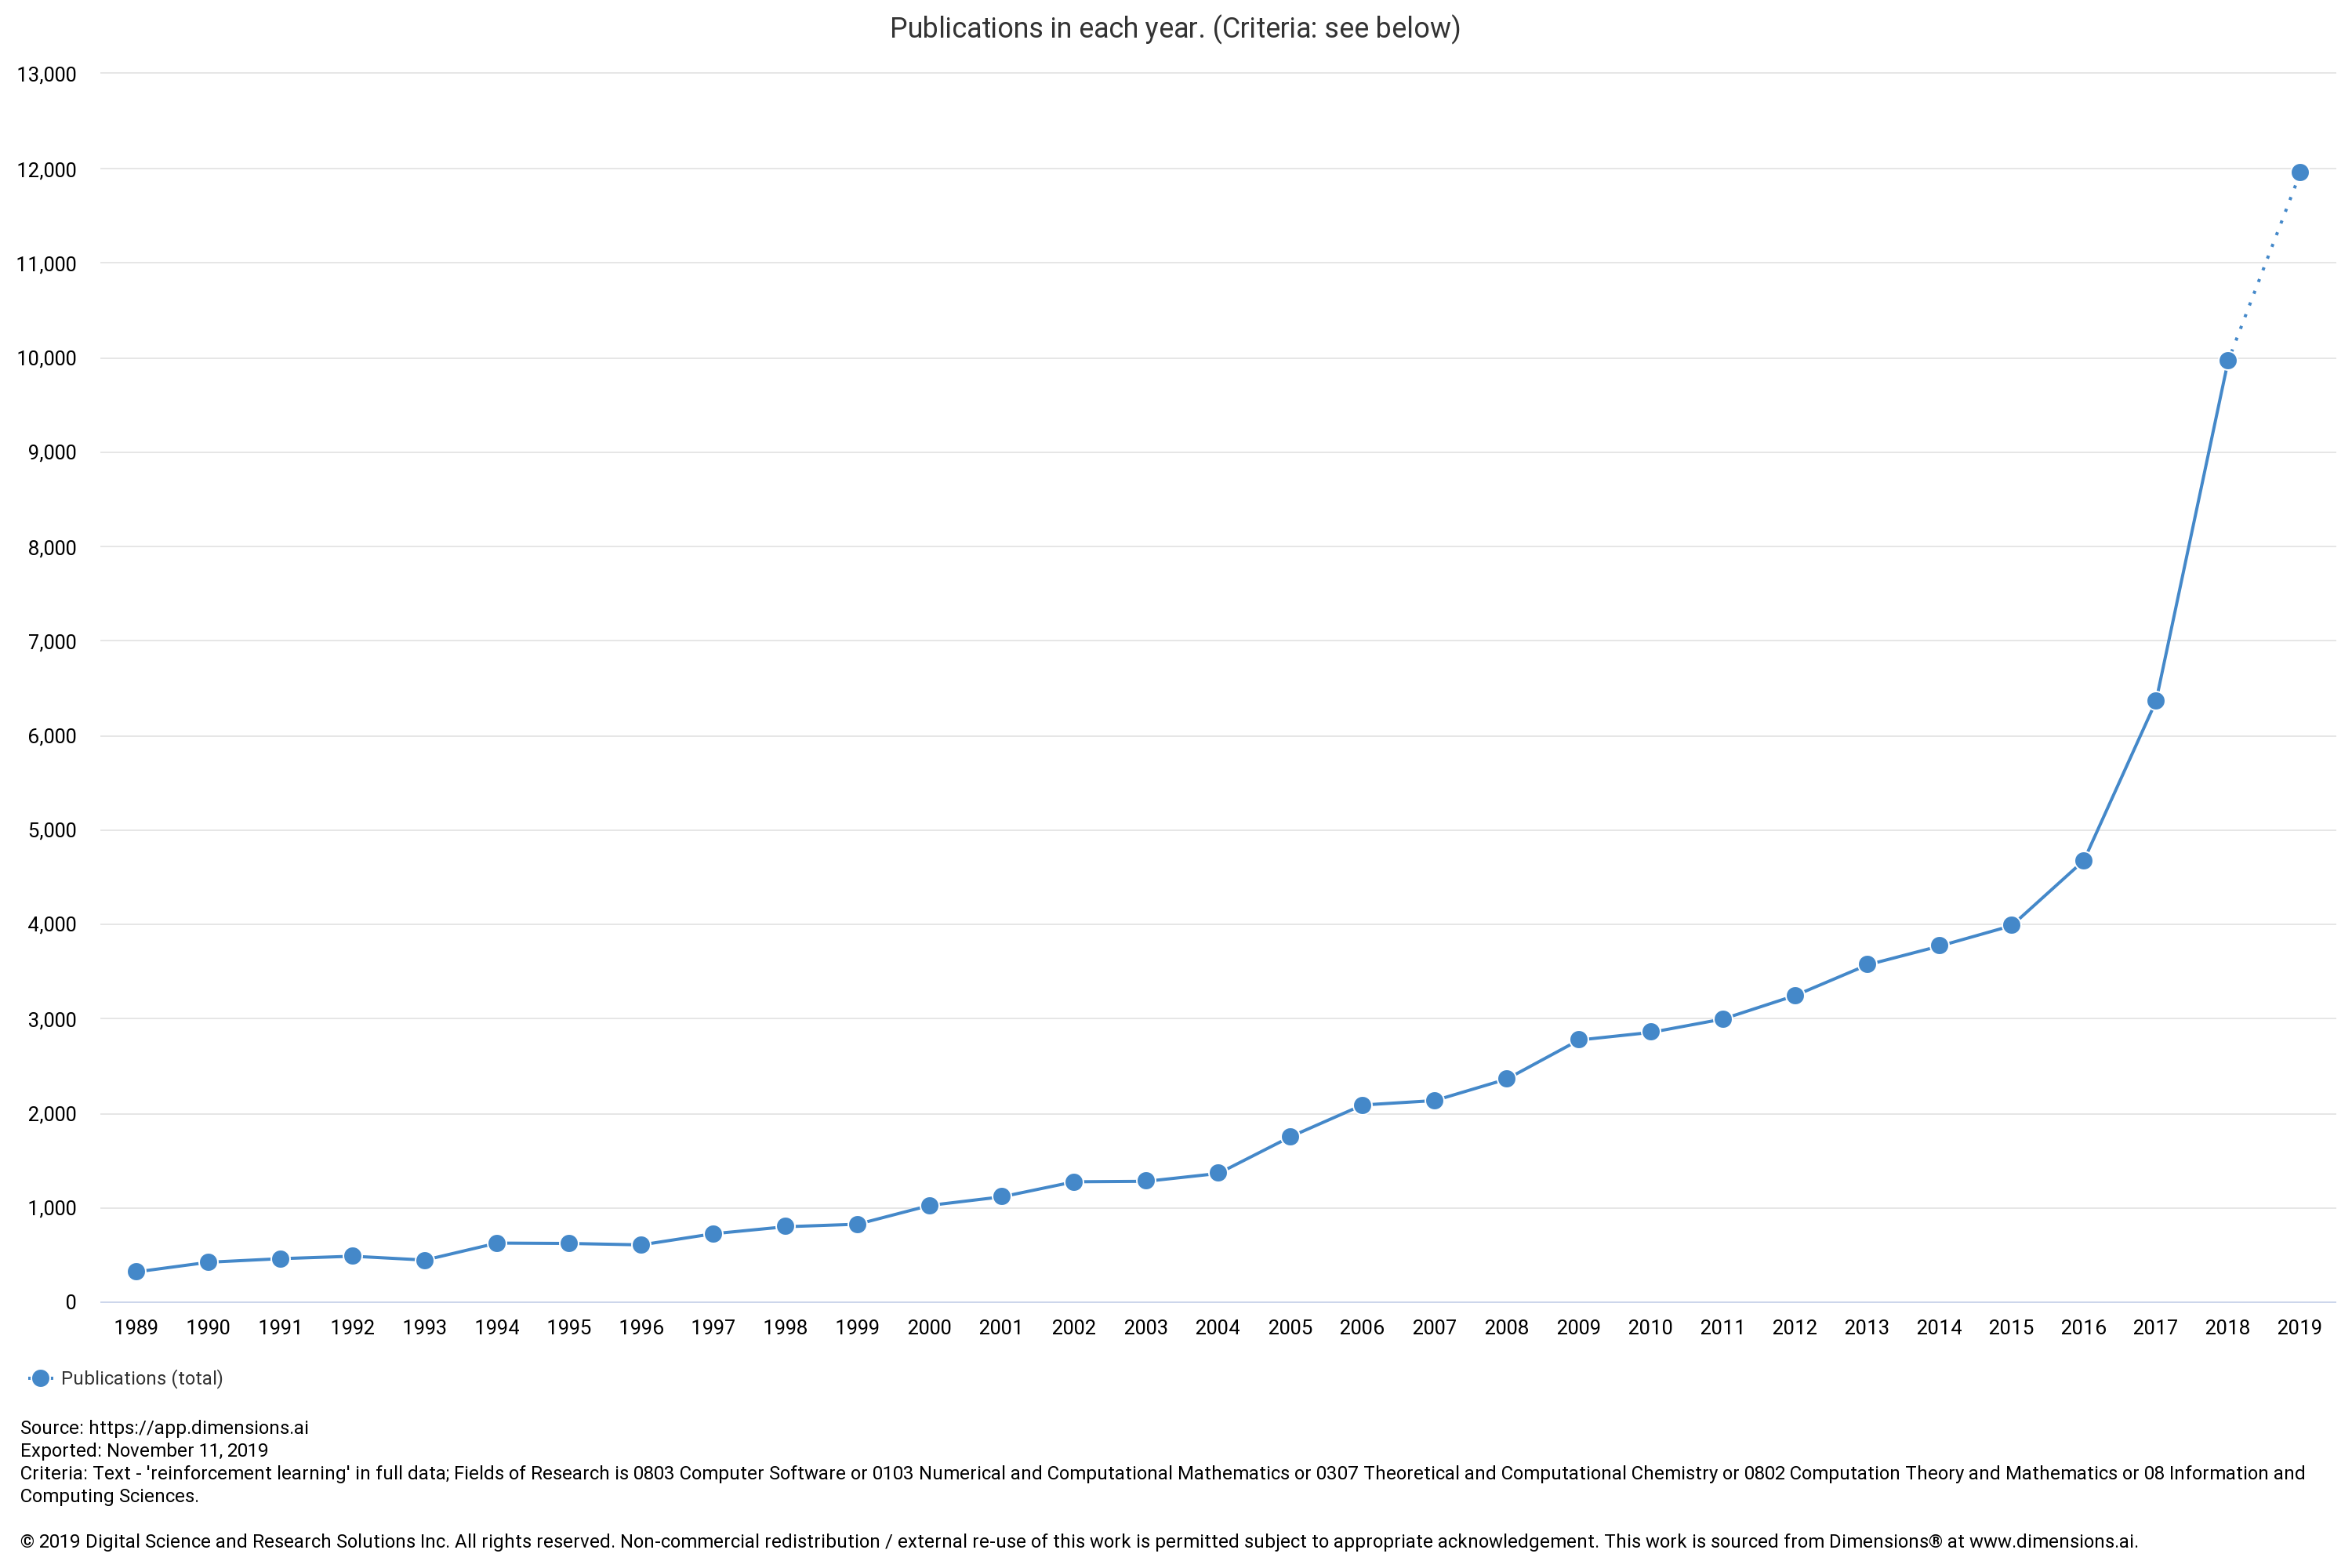
\includegraphics[width=.7 \textwidth]{conteudo/imgs/rl-publications-overview.png}
  \caption[Crescimento do número de publicações sobre RL]{Crescimento do número de publicações sobre \textit{Reinforcement Learning.}}
  \label{rl-publications-overview}
 \end{figure}


Do ponto de vista econômico, são inúmeros os usos de \textit{deep learning} no mercado. Desde ferramentas que melhoram a precisão dos sensores de precipitação por satélite e concentrando-se na redução do viés e dos alarmes falsos \cite{doi:10.1175/JHM-D-15-0075.1}, à agentes que permitem que diferentes dispositivos eletrônicos interpretem dados de multimídia não estruturados e reajam de maneira inteligente aos eventos do usuário e do ambiente \cite{dl-IoT}, o DL tem se tornado cada vez mais presente e essencial para a sociedade. Grandes setores e empresas na área da tecnologia não existiriam sem o uso dessas ferramentas.

Em relação aos impactos sociais do DL podemos mencionar a sua utilização para estimar as características socioeconômicas de regiões de 200 cidades dos Estados Unidos usando 50 milhões de imagens de cenas de rua reunidas com carros do \textit{Google Street View} \cite{Gebru13108}. O DL também teve impactos em diversas áreas da ciência, desde pesquisa em física de partículas \cite{baldi:s:w:2015}, à medicina \cite{nassif:speech-rec:2019}.

É interessante ressaltar que apesar de todos os benefícios oferecidos pela IA, alguns indivíduos notáveis como o famoso físico Stephen Hawking, e o líder da Tesla e da SpaceX Elon Musk, sugerem que a IA pode ser potencialmente muito perigosa. De fato, existem muitos aplicativos de IA que tornam nossa vida cotidiana mais conveniente e eficiente. São os aplicativos de IA que desempenham um papel crítico para garantir a segurança que Musk, Hawking e outros estavam preocupados quando proclamaram sua hesitação sobre a tecnologia. Por exemplo, se a IA for responsável por garantir a operação de nossa rede elétrica, de uma usina nuclear ou outro sistema de alto risco, e a IA for invadida ou tiver seus objetivos desalinhados com os nossos, isso poderá resultar em danos enormes \cite{Marr:AI-Danger}. 

Apesar de todo o medo ao redor dessa nova tecnologia, muitos argumentam que os mesmos são exagerados e que os benefícios oferecidos são muito maiores que os potenciais riscos, desde que sejam gerenciados adequadamente. O crescimento de pesquisas em DRL revelam seu grande potencial e benefícios para a sociedade. Reproduzir e comparar os trabalhos existentes existente e julgar com precisão as melhorias oferecidas por novos métodos é vital para sustentar esse progresso. 



% ----------------------------------------------------------

% ----------------------------------------------------------
% Abordagem proposta 
% ----------------------------------------------------------
% ----------------------------------------------------------
% Abordagem proposta 
% ----------------------------------------------------------
\chapter{Abordagem Proposta}
\label{chap:abordagem}
% ----------------------------------------------------------


No contexto de jogos digitais, treinar um agente para superar os jogadores humanos e otimizar sua pontuação pode nos ensinar como otimizar processos diferentes em uma variedade de subcampos intrigantes \cite{comi:teach:AI:DRL:2018}. Uma solução proposta na literatura, obtendo ótimos resultados, e que tem como objetivo treinar um computador pra aprender e desenvolver estratégias para jogar diferentes jogos, é o \textit{deep reinforcement learning} (DRL). 

No presente trabalho é proposto a implementação de uma inteligência artificial que, utilizando um algoritmo de \textit{deep reinforcement learning}, seja capaz de aprender a jogar diferentes jogos e desenvolver estratégias para maximizar sua pontuação.

Diante das peculiaridades e restrições do problema discutidos em \textbf{\ref{sec:descricao_do_problema}}, a biblioteca \textit{Allegro} foi escolhida como a base para a implementação dos jogos que serão apresentados ao sistema.
O \textit{Allegro} é uma biblioteca multiplataforma destinada principalmente a jogos de vídeo e programação multimídia. A biblioteca fornece rotinas de baixo nível comumente necessárias na programação de jogos, como a criação de janelas, aceitação de entrada do usuário, carregamento de dados, desenho de imagens, reprodução de sons etc \cite{allegro}.

Por fim, para auxiliar a implementação do sistema, será utilizado um \textit{Allegro Learning Enviroment}, uma ferramenta para o desenvolvimento de inteligência artificial em jogos implementados em \textit{Allegro}. Seu objetivo é oferecer uma plataforma que facilite o desenvolvimento de algoritmos de ML para jogos em \textit{Allegro}.



% section contextualização (end)
\section{\textit{Deep Learning}}


 O \textit{deep learning} (DL) é uma área do aprendizado de máquina que propõe que os computadores aprendam com a experiência, se ajustem à novas entradas de dados e compreendam o mundo em termos de hierarquia de conceitos, sendo cada conceito definido por sua relação com conceitos mais simples. 
 Ao reunir conhecimento a partir da experiência, essa abordagem evita a necessidade dos operadores humanos de especificar formalmente todo o conhecimento que o computador precisa. Além disso, a hierarquia de conceitos permite que o computador aprenda conceitos complexos, construindo-os a partir de conceitos mais simples. O \textit{deep learning} apresenta grande poder e flexibilidade a nos permitir o treinamento de computadores para cumprir tarefas específicas ao processar grandes quantidades de dados e reconhecer padrões nesses dados.


 A \textbf{Figura \ref{hierarquia-conceitos-dl}} mostra como um sitema de \textit{deep learning} representa o conceito de imagem de uma pessoa combinando conceitos mais simples, como cantos e contornos, que por sua vez são definidos em termos de arestas. 

 O mapeamento de funções de um conjunto de pixels para uma identidade de objeto é uma tarefa complicada. O algoritmo de \textit{deep learning} resolve essa dificuldade dividindo o mapeamento complicado desejado em séries de mapeamentos simples aninhados, cada um deles descrito por uma camada diferente do modelo. A entrada é apresentada na camada visível,
 em seguida, uma série de camadas ocultas extrai recursos cada vez mais abstratos da imagem. A camada de saída obtém a identidade de objeto abstrata a partir dos conceitos obtidos pelas camadas ocultas.


 \begin{figure}[h]
 \centering
 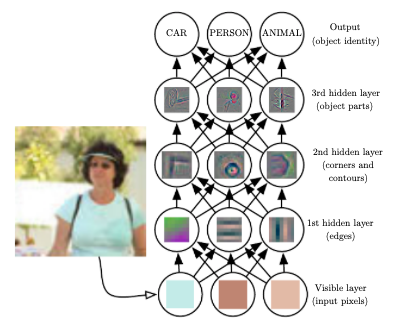
\includegraphics[width=.5 \textwidth]{conteudo/imgs/hierarquia-conceitos-dl.png}
 \caption[Ilustração de um modelo de aprendizado profundo]{Ilustração de um modelo de aprendizado profundo. Cada camada é capaz de identificar dados de complexidade crescente a partir dos pixels pasados para a camada de entrada. Imagem retirada de \cite{Goodfellow-et-al-2016}}
 \label{hierarquia-conceitos-dl}
 \end{figure}
 % \clearpage

 \section{\textit{Reinforcement Learning}} % (fold)
 \label{sec:reinforcement_learning}

 O aprendizado por reforço ou \textit{reinforcement learning} (RL) é uma abordagem computacional para entender e automatizar o aprendizado direcionado a objetivos e a tomada de decisões. O aprendizado por reforço distingue-se de outras abordagens computacionais por sua ênfase na aprendizagem de um agente apartir da interação direta com seu ambiente, sem exigir supervisão exemplar ou modelos completos do ambiente \cite{reinforcement-learning-intro-2018}.

 Em algoritmos de \textit{reinforcement learning}, o agente não é informado sobre quais ações executar, mas, em vez disso, deve descobrir quais ações geram mais recompensa, através de tentativa e erro. Em alguns casos mais interessantes, as ações podem afetar não apenas a recompensa imediata, mas também a próxima situação e, com isso, todas as recompensas subsequentes. Essas duas características - pesquisa por tentativa e erro e recompensa atrasada - são as duas características distintivas mais importantes do aprendizado por reforço.

 % O aprendizado por reforço é diferente do aprendizado supervisionado, o tipo de aprendizado estudado na maioria das pesquisas atuais no campo do aprendizado de máquina. Aprendizado supervisionado é aprender com um conjunto de treinamento de exemplos rotulados fornecidos por um supervisor externo qualificado. O objetivo desse tipo de aprendizado é o sistema extrapolar ou generalizar suas respostas para que ele atue corretamente em situações não presentes no conjunto de treinamento.
 %  % Este é um tipo importante de aprendizado, mas por si só não é adequado para aprender com a interação. Em problemas interativos, muitas vezes é impraticável obter exemplos do comportamento desejado que sejam corretos e representativos de todas as situações nas quais o agente precisa agir. Em um território desconhecido - onde se espera que a aprendizagem seja mais benéfica - um agente deve ser capaz de aprender com sua própria experiência.

 %  O aprendizado por reforço também é diferente do que os pesquisadores de aprendizado de máquina chamam de aprendizado não supervisionado, que geralmente consiste em encontrar estruturas ocultas em coleções de dados não rotulados. Os termos aprendizado supervisionado e aprendizado não supervisionado parecem classificar exaustivamente os paradigmas de aprendizado de máquina, mas não o fazem. Embora se possa ficar tentado a pensar no aprendizado por reforço como um tipo de aprendizado não supervisionado, porque não se baseia em exemplos de comportamento correto, o aprendizado por reforço está tentando maximizar um sinal de recompensa em vez de tentar encontrar uma estrutura oculta. Descobrir a estrutura na experiência de um agente certamente pode ser útil no aprendizado por reforço, mas por si só não aborda o problema do aprendizado por reforço de maximizar um sinal de recompensa. Portanto, o aprendizado por reforço é considerado como um terceiro paradigma de aprendizado de máquina, ao lado de aprendizado supervisionado, aprendizado não supervisionado e talvez outros paradigmas  \cite{reinforcement-learning-intro-2018}.

 Além do agente e do ambiente, é interessante ressaltar outros elementos importantes de um sistema de aprendizado por reforço: a \textbf{política}, o \textbf{sinal de recompensa} e a \textbf{função de valor}.

 A \textbf{política} define a maneira que o agente deve se comportar em um determinado momento. 
 Uma política é basicamente um mapeamento dos estados do ambiente para as ações a serem tomadas quando nesses estados. 
 A política em casos mais simples ter a forma de uma função simples ou uma tabela de pesquisa, enquanto em casos mais complexos pode envolver cálculos mais extensivos. 
 Em geral, as políticas podem ser estocásticas, especificando probabilidades para cada ação.

 Um \textbf{sinal de recompensa} define o objetivo de um problema de aprendizado por reforço. 
 Em cada etapa, o ambiente envia ao agente de aprendizado por reforço um único número que funciona como uma recompensa para o agente. 
 O único objetivo do agente é maximizar a recompensa total que recebe a longo prazo.
 O sinal de recompensa define, portanto, quais são os eventos bons e ruins para o agente. 
 O sinal de recompensa é a base principal para alterar a política - se uma ação selecionada pela política for seguida por uma baixa recompensa, a política poderá ser alterada para selecionar outra ação nessa situação no futuro. 
 Em geral, os sinais de recompensa podem ser funções estocásticas do estado do ambiente e das ações tomadas.

 Enquanto o sinal de recompensa indica o que é bom em um sentido imediato, uma \textbf{função de valor} especifica o que é bom a longo prazo. 
 O valor de um estado representa a quantidade total de recompensa que um agente pode esperar acumular no futuro, a partir desse estado. 
 Enquanto as recompensas determinam a conveniência imediata e intrínseca dos estados ambientais, os valores indicam a conveniência a longo prazo dos estados após levar em conta os estados que provavelmente seguirão e as recompensas disponíveis nesses estados. 
 Por exemplo, um estado sempre pode gerar uma recompensa imediata baixa, mas ainda tem um valor alto porque é seguido regularmente por outros estados que produzem recompensas altas. Ou o contrário poderia ser verdade. 

 A \textbf{Figura \ref{rl-diagram}} mostra um diagrama de aprendizagem por reforço relacionando o agente de aprendizado com o ambiente no qual ele é inserido.
 O ambiente representa o mundo pelo qual o agente se move. O ambiente nada mais é do que um sistema que toma o estado atual e a ação do agente como entrada e retorna como saída a recompensa do agente e seu próximo estado. 

 Ambientes podem ser modelados como funções que transformam uma ação executada no estado atual, no próximo estado e uma recompensa. Já os agentes podem ser modelados como funções que transformam o novo estado e recompensam na próxima ação. 
 Podemos conhecer a função do agente, mas não podemos conhecer a função do ambiente. É uma caixa preta onde só vemos as entradas e saídas. 
 % É como o relacionamento da maioria das pessoas com a tecnologia: sabemos o que faz, mas não sabemos como funciona. 
 O aprendizado por reforço representa a tentativa de um agente de aproximar a função do ambiente, para que possamos enviar ações para o ambiente de caixa preta que maximize as recompensas que ele distribui \cite{beg-guide-rl}.

 \begin{figure}[h]
  \centering
  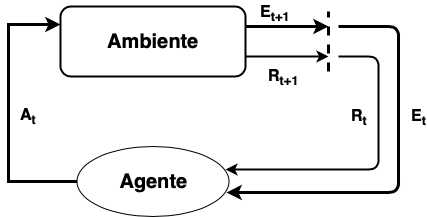
\includegraphics[width=.6 \textwidth]{conteudo/imgs/rl-diagram.png}
  \caption[Diagrama de aprendizagem por reforço]{Diagrama de aprendizagem por reforço. No \textit{loop} de \textit{feedback} acima, os subscritos indicam as etapas de tempo $t$ e $t + 1$, cada uma das quais se refere a estados diferentes: o estado no momento $t$ e o estado no momento $t + 1$. 
 % Diferente de outras formas de aprendizado de máquina - como aprendizado supervisionado e não supervisionado - o aprendizado por reforço só pode ser pensado sequencialmente em termos de pares de ação de estado que ocorrem um após o outro.
  A ação $A_t$ de um agente é determinada por sua \textbf{política}, que por sua vez é uma função que depende do estado atual do sistema $E_t$. A política de um agente tem como objetivo maximizar a \textbf{função de valor} que é calculada utilizando o \textbf{sinal de recompensa} $R_t$. O ambiente se comporta como um sistema caixa preta que transforma uma ação executada no estado atual $A_t$, no próximo estado $E_{t+1}$ e uma recompensa $R_{t+1}$
  }
  \label{rl-diagram}
 \end{figure}

 As escolhas de ação são feitas com base em julgamentos de valor.
 Buscamos ações que gerem estados de maior valor, e não de maior recompensa, porque essas ações obtêm a maior quantidade de recompensa a longo prazo. 
 % Infelizmente, é muito mais difícil determinar valores do que determinar recompensas. 
 As recompensas são basicamente dadas diretamente pelo ambiente, mas os valores devem ser estimados e re-estimados a partir das sequências de observações que um agente faz ao longo de toda a sua vida útil.


 O \textit{deep reinforcement learning} (DRL) é uma abordagem do \textit{deep learning} que, em contraste a abordagens mais tradicionais como o aprendizado supervisionado e não supervisionado, utiliza as técnicas de aprendizagem por reforço para treinar o agente. Essa abordagem consiste em fornecer ao sistema parâmetros relacionados ao seu estado e uma recompensa positiva ou negativa com base em suas ações. Nenhuma regra sobre o jogo é dada e, inicialmente, o agente não tem nenhuma informação sobre o que precisa fazer. O objetivo do sistema é descobrir e elaborar uma estratégia para maximizar sua pontuação - ou recompensa.



\section{Aplicação de DRL em um \textit{Allegro Learning Enviroment}} % (fold)
 \label{sec:allegro_learning_enviroment}

 O \textit{Arcade Learning Enviroment} é uma ferramenta de software que oferece uma interface para interagir com ambientes de jogos Atari 2600 emulados. Seu objetivo é oferecer uma plataforma que facilite o desenvolvimento de agentes de aprendizado para aprender a jogar jogos Atari. Essa ferramenta também fornece uma camada de manipulação de jogos que
 transforma cada jogo em um problema padrão de aprendizado por reforço, identificando a pontuação acumulada e se o jogo terminou. \cite{arcade-learning-enviroment}

 Inspirado na plataforma descrita acima, este trabalho visa a utilização de um \textit{Allegro Learning Enviroment}, que funcionaria de forma semelhante ao \textit{Arcade Learning Enviroment}, com a distinção de que o primeiro seria uma plataforma voltada para jogos implementados em \textit{Allegro}. O \textit{Allegro Learning Enviroment} (ALE) terá como base a ferramenta implementada por \cite{silva:amb-jd-allegro}, que oferece um ambiente facilitador ao estudo de soluções de IA aplicada em jogos. Essa ferramenta fornece funcionalidades como a exportação dos comandos básicos de um jogo, que precisam ser passados para o agente para que o mesmo tenha conhecimento dos limites físicos do ambiente no qual está inserido. Isso permite que o pesquisador não fique limitado a um jogo existente, mas possa usar qualquer jogo que ele tenha acesso ao código fonte e feito em \textit{Allegro}.

 Para o treinamento do agente, serão utilizados capturas da tela em cada estado do jogo, obtidas pelo ALE. A partir dessas imagens serão extraídas  as informações do estado atual do jogo (posição do jogador, obstáculos, etc), de forma a determinar qual a melhor ação do agente para a situação na qual ele se encontra. A utilização de capturas de tela como entradas para o agente permite que a IA seja treinada para situações em que hajam obstáculos gerados de forma aleatória. A partir dessas imagens, o agente deverá ser capaz de identificar tais obstáculos, sua localização e a melhor maneira de lidar com os mesmos.

 Em relação aos jogos nos quais o agente será treinado, a proposta é de se utilizar diferentes jogos de diferentes complexidades para avaliar o potencial do sistema. Os jogos serão obtidos de fontes de código aberto disponíveis \textit{online} ou, caso seja necessário, serão implementados com os requisitos necessário para o projeto.



 

 % [TODO]


 % \section{Modelagem matemática} % (fold)
 % \label{sec:modelagem_matemática}
 
 % section modelagem_matemática (end)





% ----------------------------------------------------------


% ----------------------------------------------------------
% Conclusoes TCC 1
% ----------------------------------------------------------
% ----------------------------------------------------------
% Contextualização em Humanidades
% ----------------------------------------------------------
\chapter{Conclusões}
\label{chap:conclusoes}
% ----------------------------------------------------------

A inteligência artificial e o aprendizado de máquina são ferramentas muito poderosas e com inúmeras aplicações práticas. A IA busca fornecer softwares que sejam capazes de realizar atividades como seres humanos para automatizar e otimizar o trabalho de rotina. Diante do grande potencial da IA, além do crescimento exponencial de pesquisa que a área vêm sofrendo, grandes empresas no mercado estão investindo na tecnologia, seja para propor novos serviços ou aprimorar produtos existentes e garantir uma vantagem competitiva no mercado.

 % Reproduzir e comparar o trabalhos existentes existente e julgar com precisão as melhorias oferecidas por novos métodos é vital para sustentar esse progresso. 
% O crescente investimento em pesquisa vem gerando IA cada vez mais

Situações do mundo real são muitas vezes complexas e apresentam problemas com um número muito grande de variáveis, o que dificulta a solução utilizando algoritmos de otimização tradicionais. Treinar um agente em jogos digitais para superar os jogadores humanos e otimizar sua pontuação pode nos ensinar como otimizar processos variados com múltiplas aplicações. Uma vez que se tenha uma IA que possa aprender a jogar e a otimizar estratégias para maximizar a pontuação de um jogo, pode-se facilmente implementar um jogo que simule uma situação real e aplicar o sistema para que este encontre a melhor resposta ou solução para um dado problema. Com isso em mente, o problema proposto nesse trabalho é o de implementar uma IA que, utilizando algoritmos de \textit{deep reinforcement learning}, seja capaz de aprender e desenvolver estratégias para jogar diferentes jogos digitais. 

A IA proposta deverá ser genérica, ou seja, capaz de aprender a jogar diferentes jogos, desde que se tenha acesso ao codigo fonte e que sejam implementados em \textit{Allegro}. Para auxiliar na implementação do sistema será utilizado um \textit{Allegro Learning Enviroment}, plataforma que irá facilitar a implementação da ferramenta para o treinamento do agente. 

Diante disso, utilizando técnicas de DRL existentes, espera-se produzir uma IA que seja flexível e que possa ser adaptada para diferentes cenários. Neste sentido, espera-se uma IA que seja genérica e capaz de ser treinada para diversos jogos. Por fim, será feita uma análise crítica dos resultados e uma comparação dos mesmos com trabalhos semelhantes realizados por outras entidades.
\clearpage
\section{Proposta de Continuidade} % (fold)
\label{sec:proposta_de_continuidade}

Este trabalho tem como continuidade o desenvolvimento do Trabalho de Conclusão de Curso II, onde haverá um maior detalhamento sobre a modelagem matemática do problema, além de especificadas as decisões de implementação da ferramenta elaborada, bem como uma análise dos resultados.

A abordagem, além do que já foi exposto, consistirá na implementação da rede neural proposta, utilizando os algoritmos DRL mencionados para o treinamento do agente. Também serão implementados (se necessário), diferentes jogos em \textit{Allegro} para a validação do sistema. Por fim, o agente será treinado em jogos simples e de baixa complexidade e serão apresentados os resultados obtidos para avaliar o potencial do sistema. Em trabalhos futuros, a ferramenta poderá também ser utilizada para o treinamento em jogos de diferentes complexidades, ampliando ainda mais o alcance do sistema.

 \section{Cronograma TCC 2}

\begin{table}[h]
	\begin{center}
		\begin{tabularx}{\textwidth}{|N|Y|Y|Y|Y|}
			\hline
			\multicolumn{1}{|N|}{Atividades}&\multicolumn{4}{|c|}{\centering{Meses}}\\
			\hline
			&Agosto&Setembro&Outubro&Novembro\\
			\hline
			Levantamento bibliográfico&X&&&\\
			\hline
			Pesquisa e implementação da rede neural proposta do trabalho&X&&&\\
			\hline
			Aplicação do estudo realizado no assunto do TCC a ser desenvolvido&X&&&\\
			\hline
			Entrega da Visão Geral do Trabalho&21/08/2020&&&\\
			\hline
			Desenvolvimento do trabalho e implementação da rede neural proposta do trabalho&X&X&&\\
			\hline
			Elaboração do corpo principal do TCC&&X&X&\\
			\hline
			Entrega do FomulárioPonto de Controle&&11/09/2020&&\\
			\hline
			Marcação da defesa&&25/09/2020&&\\
			\hline
			Ajustes finais e conclusão to trabalho implementado&&&X&\\
			\hline
			% Elaboração da conclusão e fechamento do TCC&&&X&\\
			% \hline
			Emissão da versão inicial do TCC&&&17/10/2020&\\
			\hline
			Preparação do material referente à apresentação do TCC&&&X&\\
			\hline
			Apresentação oral para banca examinadora&&&Semana de 26 a 30/10&\\
			\hline
			Ajuste no material relativo ao trabalho escrito&&&&06/11/2020\\
			\hline
		\end{tabularx}
	\end{center}
\end{table}

% section proposta_de_continuidade (end)


% ----------------------------------------------------------

% ----------------------------------------------------------
% Modelagem 
% ----------------------------------------------------------
% ----------------------------------------------------------
% Modelagem
% ----------------------------------------------------------
\chapter{Modelagem e Implementação}
\label{chap:model}
% ----------------------------------------------------------

Como mencionado no \textbf{Capítulo \ref{chap:abordagem}}, a proposta do presente trabalho consiste na implementação de um algoritmo de \textit{deep reinforcement learning} para treinar um agente que seja capaz de aprender a jogar um jogo em \textit{Allegro.} A inspiração para o mesmo vem do trabalho realizado pelo \textit{Deep Mind} e publicado no artigo \cite{play-atari-drl-deepmind}, onde foi implementado uma IA capaz de jogar diferentes jogos Atari 2600. Assim, será implementado um sistema semelhante voltado para jogos em \textit{Allegro}.

O atual capítulo consiste em uma contextualização do ambiente e sistema a ser implementado, seguido de uma elaboração da modelagem matemática da abordagem proposta no \textbf{Capítulo \ref{chap:abordagem}} e, por fim, uma discussão sobre como o sistema foi implementado.

\section{\textit{Contextualização}} % (fold)
\label{sec:contextualizacao}


\subsection{O Jogo} % (fold)
\label{sub:o_jogo}

O ambiente escolhido para treinamento do modelo foi o jogo \textit{Frogger}. A escolha do mesmo foi feita tendo em vista sua simplicidade, tendo em vista as limitações de implementação (\textbf{Seção \ref{sub:limitacoes}}). A \textbf{Figura \ref{fig:frogg}} mostra a posição inicial do jogo utilizado. O agente controla o quadrado verde iniciado no centro inferior da tela, e tem como objetivo alcançar o topo da tela sem colidir com nenhum obstáculo, os quais são iniciados com tamanho e posições aleatórias.

\begin{figure}[h]
  \centering
  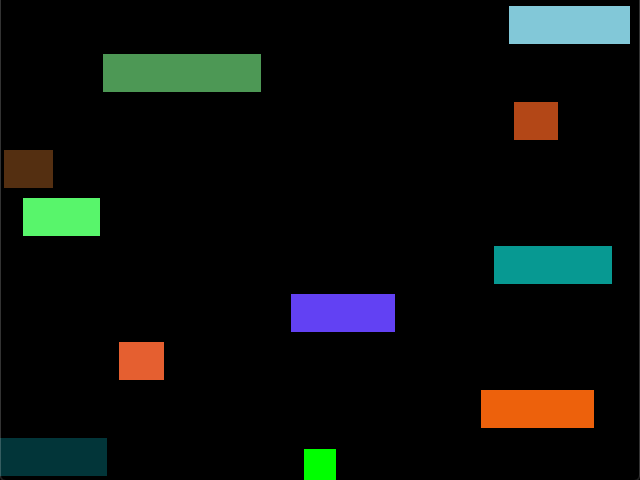
\includegraphics[width=.6 \textwidth]{conteudo/imgs/frogg_ini_state.png}
  \caption[Jogo \textit{Frogger}]{Exemplo do jogo \textit{Frogger} utilizado. O jogador controla o quadrado verde no centro inferior da tela, enquanto os outros retângulos coloridos são os obstáculos}
  \label{fig:frogg}
\end{figure} 

 As condições de parada, ou seja, os estados que constituem os estados finais do jogo são:

 \begin{itemize}
   \item Estados onde ocorra uma colisão do agente com o ambiente;
   \item Estado onde o agente atravessou o topo da tela (uma posição acima da última linha observável do jogo).
 \end{itemize}

 Por fim, as recompensas para ações durante o jogo foram definidas inicialmente da seguinte forma:

 \begin{itemize}
 	\item $r=-0.05$ caso o agente realize uma ação que o mantenha na mesma linha que se encontrava previamente. Essa recompensa negativa foi estipulada com o objetivo a desmotivar o agente a permanecer longos períodos de tempo sem progredir;
 	\item $r=1$ caso o agente realize uma ação que o aproxime verticalmente de seu objetivo;
  \item $r=-1$ caso o agente realize uma ação que o distancie verticalmente de seu objetivo;
 	\item $r=-1$ caso o agente realize uma ação que o leve a colidir com algum obstáculo (independente da direção que se movimentou);
 	\item $r=10$ caso o agente alcance seu objetivo.
 \end{itemize}

 % subsection o_jogo (end)
 
 \subsection{\textit{Allegro Learning Enviroment}} % (fold)
\label{sub:allegro_learning_enviroment}

Conforme descrito no \textbf{Capítulo \ref{chap:abordagem}}, será utilizada um \textit{Allegro Learning Enviroment} (ALE) que funcionará como intermédio entre o jogo e a IA. Essa ferramente tem como base a ferramente implementada por \cite{silva:amb-jd-allegro}, que foi modificada para atender as necessidades especificas do sistema atual. O ALE terá as seguintes funções principais:

\begin{itemize}
  \item Fornecer os valores de $\mathcal{A} = \{1,\cdots ,K\}$, que representa o conjunto de ações possíveis para o agente; 
  \item Determinar a posição da tela do jogo e realizar a captura das imagens que servirão como observações de estado para o agente;
  \item Executar um novo jogo para cada episódio de treinamento;
  \item Executar as ações estabelecidas pelo agente;
  \item Processar os dados do jogo incluindo: observação de cada instante de tempo, calcular a recompensa do atual estado do jogo, informação sobre quando um episódio é finalizado.
\end{itemize}

% subsection allegro_learning_enviroment (end)

% section reinforcement_learning (end)

\section{Modelagem Matemática} % (fold)
\label{sec:modelagem_matematica}

% \subsection{Aprendizagem por Reforço}

Como elaborado anteriormente, no aprendizado por reforço é desenvolvido um agente que irá interagir com um ambiente $\varepsilon$, nesse caso o jogo em \textit{Allegro}, a partir de uma sequência de ações, observações e recompensas.
Em cada etapa de tempo, o agente seleciona uma ação do conjunto de ações legais do jogo, $\mathcal{A} = \{1,\cdots ,K\}$. A ação é executada, modificando o estado do ambiente e pontuação do jogo.
%Em geral, $\varepsilon$ pde ser estocástico.
O estado interno do jogo não é observado pelo agente, este observa apenas uma imagem $x_t \in \mathbb{R}^d$, que é um vetor de valores de pixel brutos que representam a tela do estado atual do jogo. Além disso, o agente recebe uma recompensa $r$ que representa a alteração na pontuação do jogo.  

Em outras palavras, um agente explora um jogo, e é treinado tentando maximizar as recompensas nesse jogo. Este ciclo é ilustrado na \textbf{Figura \ref{rl-diagram-2}}.

\begin{figure}[h]
  \centering
  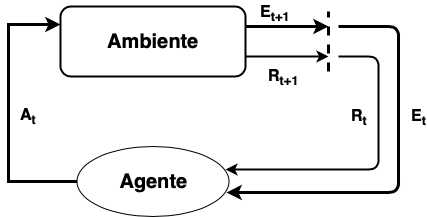
\includegraphics[width=.6 \textwidth]{conteudo/imgs/rl-diagram.png}
  \caption[Diagrama de aprendizagem por reforço]{Diagrama de aprendizagem por reforço elaborada melhor no \textbf{Capítulo \ref{chap:abordagem}}
  }
  \label{rl-diagram-2}
\end{figure}

% Em resumo, no \textit{loop} de \textit{feedback} mostrado na \textbf{Figura \ref{rl-diagram-2}}, os subscritos indicam as etapas de tempo $t$ e $t + 1$, cada uma das quais se refere a estados diferentes: o estado no momento $t$ e o estado no momento $t + 1$. 
% A ação $A_t$ de um agente é determinada por sua \textbf{política} $\pi$, que por sua vez é uma função que depende do estado atual do sistema $E_t$. A política de um agente tem como objetivo maximizar a \textbf{função de valor} $Q(s,a)$ que é calculada utilizando o \textbf{sinal de recompensa} $R_t$. O ambiente se comporta como um sistema caixa preta que transforma uma ação executada no estado atual $A_t$, no próximo estado $E_{t+1}$ e uma recompensa $R_{t+1}$

% \subsection{Processos de Decisão de Markov e a Equação de Bellman} % (fold)
% \label{sub:processos_de_decisão_de_markov}
% % subsection processo_de_decisão_de_markov (end)


É importante ressaltar que a pontuação do jogo pode depender de toda a sequência anterior de ações e observações. O \textit{feedback} sobre uma ação só pode ser recebido depois de decorridos múltiplos de intervalos de tempo. Uma vez que o agente apenas observa as imagens da tela atual, a análise do estado do jogo em que se encontra pode ser mal-representada, ou seja, é difícil para o agente compreender totalmente a situação em que se encontra apenas da tela atual $x_t$. 
Para solucionar esse problema, considera-se como um estado $s_t$ do jogo, uma sequência de ações e observações $s_t = (x_{t-n},a_{t-n},\cdots,a_{t-1},x_t)$, as quais serão utilizadas para treinar o agente, fornecendo-o um melhor contexto do estado em que se encontra. Esse formalismo dá origem a um processo de decisão de Markov (MDP), no qual cada sequência é um estado distinto. Como resultado, pode-se aplicar métodos de aprendizado por reforço padrão para MDPs, simplesmente usando a sequência completa $s_t$ como a representação do estado no tempo $t$.

Conforme descrito em \cite{play-atari-drl-deepmind}, o objetivo do agente é interagir com o jogo, selecionando ações de uma forma que maximize recompensas futuras. É feita a suposição padrão de que as recompensas futuras são descontadas por um fator de $\gamma$ por intervalo de tempo, e que o retorno descontado futuro é definido por: 
\begin{eqnarray}
	R_t=\sum_{t^{\prime}=t}^T \gamma^{t^{\prime}-t}\cdot r_{t^{\prime}}
\end{eqnarray}
onde T é o intervalo de tempo em que o jogo termina. 

A função de valor de ação ótima $Q^{*}(s, a)$ pode ser definida como o máximo retorno esperado alcançável de uma estratégia, depois de ver a sequência $s$ e se tomar alguma ação $a$:
\begin{eqnarray}
	Q^{*}(s, a)=max_\pi(\mathbb{E}[R_t | s_t=s,a_t=a,\pi])
\end{eqnarray}
onde $\pi$ é uma política que mapeia sequências para ações e $\mathbb{E}$ é a função de retorno esperado para um estado $s$ dado uma ação $a$.

A função de valor de ação ótima obedece a identidade da equação de Bellman. Essa se baseia na seguinte intuição: se o valor ótimo $Q^{*}(s_{t+1}, a_{t+1})$ da sequência $s_{t+1}$ na próxima etapa de tempo for conhecido para todas as ações possíveis ações $a_{t+1}$, então a estratégia ótima para o estado $s_t$ consiste em selecionar a ação $a_{t}$ que maximize o valor esperado futuro:
\begin{eqnarray}
	Q^{*}(s_t, a_t)= r + \gamma \cdot max(Q^{*}(s_{t+1},a_{t+1})|\forall a_{t+1})
  \label{eq:q_fun}
\end{eqnarray}

A ideia básica por trás de muitos algoritmos de aprendizagem por reforço é estimar a função de valor de ação, usando a equação de Bellman como uma atualização iterativa. Assim, dado um fator de aprendizagem $\alpha$, o valor de $Q(s,a)$, é atualizado durante o treinamento da seguinte forma:
\begin{eqnarray}
  Q_{i+1}(s_t,a_t) = Q(s_t,a_t) + \alpha[r + \gamma\cdot max_{a_{t+1}}Q(s_{t+1},a_{t+1}) - Q(s_t,a_t)]
  \label{eq:qlearning}
\end{eqnarray}

sendo que a subtração de $\gamma\cdot max_{a_{t+1}}Q(s_{t+1},a_{t+1})$ por $Q(s_t,a_t)$ é realizada para normalizar a atualização. 

Essa atualização dos valores da função de valor $Q$, permite que o algoritmo convirja para a função de ação ótima $Q_i \rightarrow Q^*$, com $i\rightarrow\infty$ \cite{sutton-barto-rl-intro}. Na prática, essa abordagem é totalmente impraticável, pois a função valoração é estimada separadamente para cada sequência, sem nenhuma generalização. Em vez disso, é comum usar um aproximador de função para estimar a função de valor de ação, $Q(s,a;\theta_t) \approx Q^*(s,a)$. Este aproximador toma a forma de uma rede neural, conhecida como uma \textit{Q-network}, onde $\theta_t$ refere-se aos parâmetros da rede neural (ou seja, os pesos e bias da rede). Assim, se os pesos são atualizados após cada passo de tempo, então chegamos ao conhecido algoritmo de \textit{Q-learning} \cite{Watkins-Dayan-Qlearning}. O valor de $\theta_t$ por sua vez pode ser atualizado conforme a \textbf{Equação \ref{eq:theta}}:
\begin{eqnarray}
  \theta_t = \theta_t + \alpha(r + \gamma\cdot max_{a_{t+1}}Q(s_{t+1},a_{t+1}) - Q(s_t,a_t))\nabla_\theta Q(s_t,a_t)
  \label{eq:theta}
\end{eqnarray}

Por fim, considerando a iteração de treinamento do agente usando \textit{Q-learning}, a política de seleção de ação é baseada apenas no valor máximo de $Q$ em qualquer estado dado. É concebível que, dada a inicial natureza estocástica do ambiente, o agente inicialmente tome decisões “ruins”. No entanto, como o agente nunca explorou ações melhores, ele pode interpretar que as decisões ruins tomadas inicialmente são boas e, daquele momento em diante, tomar somente aquelas decisões. Da mesma forma, mesmo que o agente tome ações iniciais ``boas'' ele pode acabar desenvolvendo uma política que prenda o agente em ótimos locais, ou seja, a ação determinada pela política é boa a curto prazo, mas a longo prazo ela é inferior ou até ruim. Esta política de seleção de ação é chamada de política gulosa.

Para evitar esses problemas, o agente deve explorar o maior número possível de estados e ações. Infelizmente, para problemas com um número muito grande de estados, explorar todos os estados e ações possíveis se torna impraticável. A política \textit{epsilon-greedy} na aprendizagem por reforço é basicamente a mesma que a política gulosa, exceto que há um valor épsilon que define uma probabilidade $1-\epsilon$ de uma ação ser escolhida aleatoriamente ao invés de definida pelo atual modelo. Dessa forma, o algoritmo força o agente a explorar diversos estados e ações, mesmo que estes não sejam a princípio recomendados pela função de valor $Q$. Dado um número suficientemente grande de ações, o agente terá explorado uma quantidade de estados suficiente para determinar uma política satisfatória. Essa abordagem permite também que o valor de $\epsilon$ seja atualizado e reduzido com o tempo de forma a permitir que o algoritmo se concentre mais em explorar as melhores soluções que encontrou. 

% section modelagem_matemática (end)

\section{Implementação} % (fold)
\label{sec:implementacao}

A modelagem descrita na \textbf{Seção \ref{sec:modelagem_matematica}}, fornece uma modelagem da rede neural proposta. O sistema nada mais é do que uma \textit{Deep Q Network} (DQN), que é constituída por uma \textit{Deep Neural Network} \cite{Goodfellow-et-al-2016} que utiliza a técnica de \textit{Q-learning}, onde cada nó de saída da rede corresponde à uma possível ação do agente. No entanto, um simples algoritmo usando o método descrito não converge para uma solução satisfatória. Nessa seção serão vistas algumas modificações para o algoritmo que o fará obter melhores resultados.

\subsection{\textit{Experience Replay}} % (fold)
\label{ssub:experience_replay}

Foi aplicada a técnica conhecida como \textit{Experience Replay} \cite{Lin1992ReinforcementLF}, onde as experiências do agente em cada passo de tempo, são armazenadas em um \textit{replay buffer}, que nada mais é do que uma lista de tuplas, cada tupla contendo o estado atual, a ação tomada, a recompensa obtida, e o próximo estado alcançado $(s_t,a_t,r_t,s_{t+1})$. Para treinar a DQN, recupera-se aleatoriamente um pequeno lote do \textit{replay buffer}, o qual é usado como dado de treinamento. A \textbf{Figura \ref{fig:exp_rep}} mostra o processo descrito.


\begin{figure}[h]
  \centering
  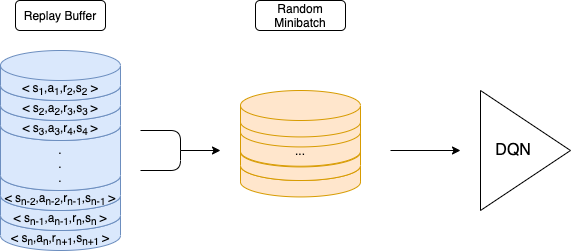
\includegraphics[width=.7 \textwidth]{conteudo/imgs/experience_replay.png}
  \caption[\textit{Experience Replay}]{Exemplo do processo de seleção de dados de treinamento. O histórico de estados, ações e recompensas obtido é salvo em um \textit{replay buffer}. Para treinar o agente, o algoritmo seleciona aleatoriamente um conjunto de amostras (\textit{minibatch}) de tamanho pré-definido que servirão como dados de treinamento da rede}
  \label{fig:exp_rep}
\end{figure} 

O \textit{buffer} implementado dessa forma é uma fila FIFO (\textit{First in, first out}), ou seja, quando ele atingir seu tamanho máximo, as novas entradas irão substituir as entradas mais antigas de forma a sempre manter o conjunto de dados mais atualizado. Além disso, antes de se inicializar o treinamento, o \textit{buffer} é inicializado com um tamanho mínimo, inicializado com amostras obtidas por um agente com política de ação aleatória.

O objetivo da alocação dos dados dessa forma é de fornecer à rede uma melhor distribuição de informação para o aprendizado. Um algoritmo de aprendizado simples recebe os dados de treinamento na mesma ordem em que são observados. Isso pode introduzir ao agente padrões ou correlações indesejadas, que podem afetar o processo de aprendizado do algoritmo. Assim, ao passar as observações de forma aleatória, a eficiência do algoritmo é melhorada. 


% subsubsection experience_replay (end)


\subsection{Pré-processamento de Imagens} % (fold)
\label{sub:preprocessamento}

Para treinar uma rede neural apartir de capturas de tela em cada instante do jogo, os dados de cada observação são extraídos dos pixels brutos exibidos. Um problema de utilizar imagens estáticas como observações é que isso limita a quantidade de informação que pode ser obtida do estado do jogo: não é possível determinar a velocidade ou direção na qual um objeto está se movendo. Para contornar essa situação, pode-se redefinir um estado como sendo um conjunto de $n$ instantes de tempo, como mencionado na \textbf{Seção \ref{sec:modelagem_matematica}}. 

Dado que a tela do jogo representa uma janela de $640\times480$ pixels, pode-se converter isso para um vetor de pixels RGB com dimensões $640\times480\times3$. Uma vez definido o estado como um conjunto de $n=4$ instantes, temos um vetor de entrada para rede neural de $640\times480\times3\times4=3686400$. Considerando que cada iteração do algoritmo deverá analisar um vetor desse tamanho, o custo computacional do treinamento do modelo é extremamente alto. Felizmente o vetor de entrada pode ser reduzido consideravelmente removendo algumas informações desnecessárias. Primeiramente, do ponto de vista do agente, a variação de cores do jogo é irrelevante. Sendo assim, pode-se converter a imagem para cinza, reduzindo o tamanho da matriz da imagem original de $640\times480\times3$ para $640\times480$. Por fim, podemos reduzir o tamanho dessa imagem, tendo em vista que informações redundantes de uma tela grande não são necessárias para treinamento do modelo. A \textbf{Figura \ref{fig:pross_imgs}} mostra o tratamento de uma imagem antes de ela ser adicionada ao estado que servirá de entrada para a rede.

\begin{figure}[h]
  \centering
  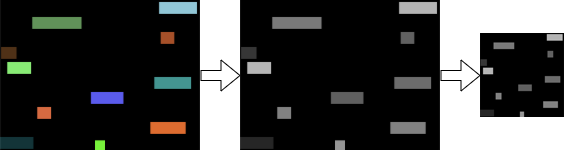
\includegraphics[width=.9 \textwidth]{conteudo/imgs/reducao_imgs.png}
  \caption[Processamento de Imagens]{Processamento das capturas de tela realizado antes das mesmas serem passadas como entradas para o treinamento da rede. Primeira imagem na esquerda é um exemplo da captura original, seguindo da mesma imagem transformada para cinza e por fim a imagem reduzida que será convertida para um vetor de pixels a ser passado como entrada para o modelo}
  \label{fig:pross_imgs}
\end{figure} 

Com isso, considerando uma redução para uma imagem final de $84\times84$ pixels, obtém-se um estado formado por um vetor de tamanho $84\times84\times4=28224$. Apesar do vetor final ainda apresentar um tamanho considerável, foi alcançado uma redução de $99.23\%$ na entrada do modelo, aliviando consideravelmente o custo computacional do sistema.

% subsection préprocessamento (end)

\subsection{\textit{Dueling Q Network}} % (fold)
\label{sub:rede_neural_dupla}

O problema do aprendizado por DQN está ligado à definição da sua função de valor. Da \textbf{Equação \ref{eq:q_fun}} temos:
$$Q^{*}(s_t, a_t)= r + \gamma \cdot max(Q^{*}(s_{t+1},a_{t+1})|\forall a_{t+1})$$

O problema da equação acima surge com o valor máximo. Esta parte da equação deve estimar o valor das recompensas para ações futuras se a ação $a$ for tomada a partir do estado atual $s_t$. O problema é que em muitos ambientes, a existência de um ruído aleatório, ou seja, uma variância no valor da recompensa, é inevitável. Assim, à medida que um agente explora um ambiente, ele não está observando diretamente $r$ ou $r_{futuro}$, mas algo como $r + \epsilon$, onde $\epsilon$ é o ruído ou o a variância da recompensa. Em tal ambiente, depois de jogar o jogo repetidamente, esperaríamos que a rede aprendesse a fazer estimativas imparciais do valor esperado das recompensas $E[r]$. Com isso, basta à rede escolher as melhores ações para recompensas atuais e futuras, apesar da presença de ruído.

É aqui que a operação de máximo é um problema: ela produz estimativas tendenciosas das recompensas futuras, não as estimativas imparciais de que necessitamos para obter os melhores resultados.
Considere o ambiente exemplificado pela \textbf{Figura \ref{fig:dqn_bias}} \cite{ThomasAndrew:adv_ml}. O agente começa no estado A e em cada estado pode mover-se para a esquerda ou direita. Os estados C e E são estados terminais. O jogo termina quando esses pontos são alcançados. Os valores de $r$ são as recompensas que o agente recebe ao fazer a transição de um estado para outro.

\begin{figure}[h]
  \centering
  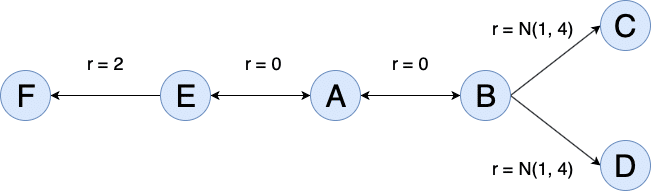
\includegraphics[width=.9 \textwidth]{conteudo/imgs/dqn_bias.png}
  \caption[\textit{Deep Q Network} bias]{Exemplo de um jogo que causa bias em uma DQN. O agente começa no estado A e em cada estado pode mover-se para a esquerda ou direita. Os estados C e E são estados terminais. O jogo termina quando esses pontos são alcançados. Os valores de $r$ são as recompensas que o agente recebe ao fazer a transição de um estado para outro. Figura extraída de \cite{ThomasAndrew:adv_ml}}
  \label{fig:dqn_bias}
\end{figure} 

Todas as recompensas são determinísticas, exceto as recompensas durante a transição dos estados B para C. As recompensas para essa transição é retirada aleatoriamente de uma distribuição normal com uma média de 1 e um desvio padrão de 4.

Sabemos as recompensas esperadas, $E[r]$ de qualquer ação de B para C é 1. No entanto, há uma variância associada à essas recompensas. Independentemente disso, em média, o agente deve aprender idealmente a sempre se mover para a esquerda de A, em direção a D e finalmente E, onde r sempre é igual a 2. No entanto, devido a função de máximo utilizada para calcular a função de valor, sempre é obtido o valor máximo dos sorteios aleatórios das recompensas e, com isso, o algoritmo tende a ser positivamente tendencioso e não dá uma indicação verdadeira dos valores esperados das recompensas para um movimento nesta direção (ou seja, 1). Como tal, um agente que usa a metodologia de \textit{Q-learning} não escolherá a ação ideal de A (ou seja, mover para a esquerda), mas tenderá a mover para a direita.

A solução para este problema foi proposta por \cite{vanhasselt2015deep}, e consiste na implementação de duas redes neurais, mas somente uma rede primária é treinada à cada iteração, enquanto a segunda rede, chamada de rede objetivo, é treinada com menos frequência. Esse processo ajuda a estabilizar os pesos da rede objetivo.

A arquitetura conhecida como \textit{Dueling Q}, é uma melhoria para a rede neural dupla. Utiliza-se a mesma metodologia de uma rede alvo e primária, com atualizações periódicas ou combinação dos pesos da rede alvo com os pesos da rede primária. No entanto, ele incorpora dois conceitos importantes na arquitetura da rede. Estas são as funções de vantagem e valor:

\begin{itemize}
  \item \textbf{Função de vantagem $A(s,a)$}: A função de vantagem é o benefício relativo de escolher uma determinada ação no estado $s$ sobre as outras ações possíveis no mesmo estado.
  \item \textbf{Função de valor V(s)}: A função de valor é o valor de estar no estado s, independente dos benefícios relativos das ações nesse estado
\end{itemize}

A função $Q(s,a)$ se torna então, uma adição dessas duas funções:

\begin{eqnarray}
  Q(s,a) = V(s) + A(s,a)
\end{eqnarray}

A motivação de dividir essas duas funções explicitamente na arquitetura é que pode haver estados inerentemente bons ou ruins para o agente estar, independentemente do benefício relativo de quaisquer ações nesse estado. Por exemplo, em um determinado estado, todas as ações podem fazer com que o agente "morra" em um jogo - este é um estado inerentemente ruim de se estar, e não há necessidade de desperdiçar recursos computacionais tentando determinar a melhor ação neste estado . O inverso também pode ser verdadeiro. Idealmente, esta “divisão” em função de vantagem e função de valor deve ser aprendida implicitamente durante o treinamento. No entanto, a arquitetura \textit{Dueling Q} torna essa divisão explícita, o que atua para melhorar o treinamento.

\subsection{Arquitetura Final} % (fold)
\label{ssub:arquiterura_final}

De acordo com as especificações descritas acima, a arquitetura final do modelo pode ser observada na \textbf{Figura \ref{fig:diagrama_rede}}. Pode-se observar que na arquitetura implementada, foram utilizadas camadas comuns de redes neurais convolucionais que realizam o processamento de imagens. A saída dessas camadas é então achatada e rede então se bifurca em um fluxo de função de valor $V(s)$ e um fluxo de função de vantagem $A(s,a)$. A saída desses fluxos separados é então agregada em uma camada especial, antes de finalmente produzir os valores Q da rede.

\begin{figure}[h]
  \centering
  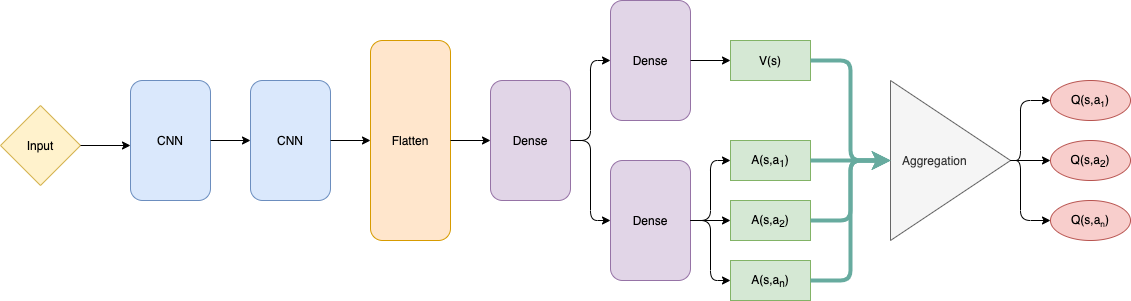
\includegraphics[width=1 \textwidth]{conteudo/imgs/diagrama_rede.png}
  \caption[Diagrama da arquitetura final da rede implementada]{Diagrama da arquitetura final da rede implementada}
  \label{fig:diagrama_rede}
\end{figure} 

A partir da arquitetura descrita acima, os \textbf{Algoritmos \ref{alg:main}} e \textbf{\ref{alg:train}} mostram o pseudocódigo do sistema implementado. O \textbf{Algoritmo \ref{alg:main}} mostra o corpo da função principal, enquanto o \textbf{Algoritmo \ref{alg:train}} descreve a função de treinamento do modelo.

\begin{algorithm}[H]
    \SetAlgoLined
    Inicializa o ambiente\\
    Inicializa a rede primária\\
    Inicializa a rede objetivo\\

    \For{episodio = 1:NUM\_EPISODIOS }{
      \While{jogo não termina}{
        ação $\leftarrow$ modelo.obtemAcao(estado,$\epsilon$)\\
        proximaObservacao, recompensa, fim $\leftarrow$ ambiente.executaAcao(ação)\\
        proximoEstado $\leftarrow$ obtemEstado(estado,proximaObservacao)\\[.3cm]

        experienceReplay.adicionaTupla(estado,ação,recompensa,proximoEstado,fim)\\[.3cm]

        treinaModelo()
      }
    }
   \caption{Corpo Principal}
   \label{alg:main}
  \end{algorithm}

  \begin{algorithm}[H]
    \SetAlgoLined
    $<s_t,a_t,r_t,s_{t+1},fim>$batch  $\leftarrow$ experienceReplay.obtemBatch()\\
    \eIf{fim}{
      $y \leftarrow r_t$
    }
    {
      $y \leftarrow r_t + \gamma\cdot max_{a_{t+1}}Q(s_{t+1},a_{t+1})$
    }

    \# Gradiente descendente\\
    $\Delta\theta\leftarrow\frac{\partial}{\partial\theta}(y - Q(s,a))^2$\\[.3cm]

    Atualiza os pesos da rede
   \caption{treinaModelo}
   \label{alg:train}
  \end{algorithm}

% subsubsection arquiterura_final (end)


% subsection rede_neural_dupla (end)


\subsection{Limitações} % (fold)
\label{sub:limitacoes}

A implementação do sistema apresentado enfrentou uma série de limitações que fogem do alcance do desenvolvedor. Os desafios encontrados durante a implementação, assim como as soluções para circunver estes problemas, quando possível, são descritas abaixo.

\subsubsection{Tempo de Treinamento e Limitações de Hardware} % (fold)
\label{subsub:tempo_de_treinamento_e_limitações_de_hardware}

O principal obstáculo enfrentado foi o tempo de treinamento do sistema. Devido a complexidade e número de entradas do problema, o modelo pode levar dias ou semanas para alcançar uma política ótima. Como mencionado anteriormente, cada estado é formado por quatro imagens constituindo os quatro últimos instante do jogo. Mesmo após a conversão para cinza e compressão das imagens de $640\times480$ para $84\times84$ pixels, isso ainda deixa cada estado com um vetor de entrada de tamanho $84\times84\times4=28224$. Tudo isso considerando um tamanho de tela bem modesto e um jogo sem informações muito complexas (quando comparado com um jogo 3D por exemplo).

Esses problemas são agravados ainda mais devido às limitações do hardware onde o sistema foi implementado. A máquina utilizada possui as seguintes especificações:

\begin{itemize}
  \item MacBook Air 2015;
  \item Processador: 1.6 GHz Dual-Core Intel Core i5;
  \item Memória: 4 GB 1600 MHz DDR3;
  \item Sistema Operacional: macOS Catalina | Windows 10.
\end{itemize}

Como pode ser observado, trata-se de uma máquina com poder computacional limitado, com relativamente pouca memória, um processador bastante simples e sem uma placa de vídeo dedicada. Todas essas limitações acabam levando à um tempo de treinamento ainda maior.

% subsection tempo_de_treinamento_e_limitações_de_hardware (end)

\subsubsection{Integração do Sistema com o Jogo em \textit{Allegro}} % (fold)
\label{subsub:integração_do_sistema_com_o_jogo}

Como mencionado no \textbf{Capítulo \ref{chap:abordagem}} e em \ref{sub:allegro_learning_enviroment}, a comunicação entre a IA, implementada em \textit{Python}, e o jogo, implementado em C, é realizada através de um \textit{Allegro Learning Enviroment} (ALE). No entanto, como o ALE também é implementado em \textit{Python}, a integração dos dois sistemas apresenta algumas limitações.

Primeiramente, o cálculo da recompensa seria, idealmente, calculado pelo programa do jogo e passado para o ALE. No entanto, qualquer saída do programa em C só é recebida pelo ALE uma vez que o programa é finalizado ao fim de um episódio. Isso inviabiliza o calculo em tempo real de qualquer estado que não sejam os estados iniciais ou finais. Por esse motivo o calculo das recompensas de cada estado deve ser feito pela ALE, o qual é realizado através um simples registro da posição do agente no jogo.

Outro problema que surge da integração da ALE com o o jogo é o processamento das imagens e que, por sua vez, acaba exacerbando ainda mais o problema de tempo de treinamento descrito em \ref{subsub:tempo_de_treinamento_e_limitações_de_hardware}. Ao iniciar um novo episódio, o programa em C leva alguns instantes para ser lançado e ter seu estado inicial renderizado. Portanto, para garantir que a observação do estado inicial do jogo seja realizada propriamente, a ALE aguarda $0.1s$ para garantir que o programa foi inicializado propriamente e $0.2s$ após o jogo ser concluído. Esse tempo torna-se considerável a medida que o número de episódios de treinamento aumentam. Um treinamento com dez mil episódios, por exemplo, recebem um aumento de cerca de $50$ minutos. 

Além disso, os jogos em \textit{Allegro} devem ter seus dados processados manualmente. A \textbf{Figura \ref{fig:process_img}} mostra um diagrama que indica todos os passos do processamento de dados necessários para gerar as informações de cada estado do jogo.

\begin{figure}[h]
  \centering
  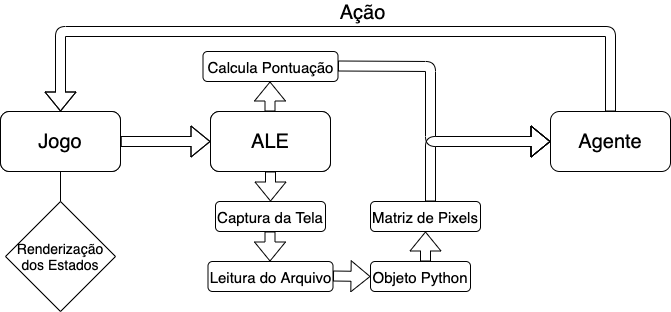
\includegraphics[width=.8 \textwidth]{conteudo/imgs/processamento_imgs.png}
  \caption[Diagrama de processamento de imagens]{Diagrama mostrando como as informações de cada estado são processadas antes de serem passadas para a IA. Isso inclui executar o programa em C, transmitir os comandos de ação do agente para o jogo, renderizar as imagens em cada instante do jogo, realizar a captura de tela, acessar os arquivos onde essas imagens foram salvas, transformar os dados desse arquivo para um objeto em \textit{Python}, transformar o objeto em uma matriz com os dados da imagem para somente então os mesmos serem passados para o modelo a ser treinado}
  \label{fig:process_img}
\end{figure} 

Jogos em Atari 2600 que possuem um emulador em \textit{Python} que são capazes de gerar um vetor de observação que contém os dados de cada instante do jogo sem a necessidade de renderizar as imagens do mesmo \cite{brockman2016openai}. O mesmo não pode ser dito para os jogos em \textit{Allegro}. Para obter as observações dos estados do jogo, deve-se executar o programa em C, renderizar cada estado do jogo e realizar a captura de tela dos mesmos, e realizar o processamento dessas imagens antes desses dados serem passados para a IA. Todo o processo deve ser realizado para cada instante que deseja-se observar e calcular uma ação. Para evitar que o alto tempo de processamento dos dados leve a alguma perda de informações que prejudique o treinamento (como o agente permanecer inativo por um longo período de tempo enquanto calcula o próximo movimento), o jogo foi alterado de forma que cada quadro (\textit{frame}) do jogo seja atualizado somente quando o agente realizar uma ação. Esse formato de implementação acaba constituindo um \textit{trade-off}: a perda de informações do agente é minimizada, mas o tempo de execução de cada episódio aumenta.

% subsection integração_do_sistema_com_o_jogo_em_tex (end)

% subsection limitações (end)
% section implementação (end)

% ----------------------------------------------------------


% % ----------------------------------------------------------
% % Introdução (exemplo de capítulo sem numeração, mas presente no Sumário)
% % ----------------------------------------------------------
% \chapter{Introdução}
% % ----------------------------------------------------------

% Este documento e seu código-fonte são exemplos de referência de uso da classe
% \textsf{abntex2} e do pacote \textsf{abntex2cite}. O documento 
% exemplifica a elaboração de trabalho acadêmico (tese, dissertação e outros do
% gênero) produzido conforme a ABNT NBR 14724:2011 \emph{Informação e documentação
% - Trabalhos acadêmicos - Apresentação}.

% A expressão ``Modelo Canônico'' é utilizada para indicar que \abnTeX\ não é
% modelo específico de nenhuma universidade ou instituição, mas que implementa tão
% somente os requisitos das normas da ABNT. Uma lista completa das normas
% observadas pelo \abnTeX\ é apresentada em \citeonline{abntex2classe}.

% Sinta-se convidado a participar do projeto \abnTeX! Acesse o site do projeto em
% \url{http://www.abntex.net.br/}. Também fique livre para conhecer,
% estudar, alterar e redistribuir o trabalho do \abnTeX, desde que os arquivos
% modificados tenham seus nomes alterados e que os créditos sejam dados aos
% autores originais, nos termos da ``The \LaTeX\ Project Public
% License''\footnote{\url{http://www.latex-project.org/lppl.txt}}.

% Encorajamos que sejam realizadas customizações específicas deste exemplo para
% universidades e outras instituições --- como capas, folha de aprovação, etc.
% Porém, recomendamos que ao invés de se alterar diretamente os arquivos do
% \abnTeX, distribua-se arquivos com as respectivas customizações.
% Isso permite que futuras versões do \abnTeX~não se tornem automaticamente
% incompatíveis com as customizações promovidas. Consulte
% \citeonline{abntex2-wiki-como-customizar} para mais informações.

% Este documento deve ser utilizado como complemento dos manuais do \abnTeX\ 
% \cite{abntex2classe,abntex2cite,abntex2cite-alf} e da classe \textsf{memoir}
% \cite{memoir}. 

% Esperamos, sinceramente, que o \abnTeX\ aprimore a qualidade do trabalho que
% você produzirá, de modo que o principal esforço seja concentrado no principal:
% na contribuição científica.

% Equipe \abnTeX 

% Lauro César Araujo

% % ----------------------------------------------------------
% % PARTE
% % ----------------------------------------------------------
% \part{Preparação da pesquisa}
% % ----------------------------------------------------------

% % ---
% % Capitulo com exemplos de comandos inseridos de arquivo externo 
% % ---
% \include{abntex2-modelo-include-comandos}
% % ---

% \chapter{Conteúdos específicos do modelo de trabalho acadêmico}\label{cap_trabalho_academico}

% \section{Quadros}

% Este modelo vem com o ambiente \texttt{quadro} e impressão de Lista de quadros 
% configurados por padrão. Verifique um exemplo de utilização:

% \begin{quadro}[htb]
% \caption{\label{quadro_exemplo}Exemplo de quadro}
% \begin{tabular}{|c|c|c|c|}
% 	\hline
% 	\textbf{Pessoa} & \textbf{Idade} & \textbf{Peso} & \textbf{Altura} \\ \hline
% 	Marcos & 26    & 68   & 178    \\ \hline
% 	Ivone  & 22    & 57   & 162    \\ \hline
% 	...    & ...   & ...  & ...    \\ \hline
% 	Sueli  & 40    & 65   & 153    \\ \hline
% \end{tabular}
% \fonte{Autor.}
% \end{quadro}

% Este parágrafo apresenta como referenciar o quadro no texto, requisito
% obrigatório da ABNT.
% Primeira opção, utilizando \texttt{autoref}: Ver o \autoref{quadro_exemplo}. 
% Segunda opção, utilizando  \texttt{ref}: Ver o Quadro \ref{quadro_exemplo}.

% % ----------------------------------------------------------
% % PARTE
% % ----------------------------------------------------------
% \part{Referenciais teóricos}
% % ----------------------------------------------------------

% % ---
% % Capitulo de revisão de literatura
% % ---
% \chapter{Lorem ipsum dolor sit amet}
% % ---

% % ---
% \section{Aliquam vestibulum fringilla lorem}
% % ---

% \lipsum[1]

% \lipsum[2-3]

% % ----------------------------------------------------------
% % PARTE
% % ----------------------------------------------------------
% \part{Resultados}
% % ----------------------------------------------------------

% % ---
% % primeiro capitulo de Resultados
% % ---
% \chapter{Lectus lobortis condimentum}
% % ---

% % ---
% \section{Vestibulum ante ipsum primis in faucibus orci luctus et ultrices
% posuere cubilia Curae}
% % ---

% \lipsum[21-22]

% % ---
% % segundo capitulo de Resultados
% % ---
% \chapter{Nam sed tellus sit amet lectus urna ullamcorper tristique interdum
% elementum}
% % ---

% % ---
% \section{Pellentesque sit amet pede ac sem eleifend consectetuer}
% % ---

% \lipsum[24]

% % ----------------------------------------------------------
% % Finaliza a parte no bookmark do PDF
% % para que se inicie o bookmark na raiz
% % e adiciona espaço de parte no Sumário
% % ----------------------------------------------------------
% \phantompart

% % ---
% % Conclusão
% % ---
% \chapter{Conclusão}
% % ---

% \lipsum[31-33]